\documentclass[fontset=none]{ctexbeamer}
\usepackage{amsmath}
\usepackage{amssymb}
\usepackage{fontspec}
\usepackage{graphicx}

\usetheme{Singapore}
\usefonttheme{serif}

\setmainfont{Source Serif Pro}
\setsansfont{Source Sans Pro}[Scale=MatchLowercase]
\setmonofont{Source Code Pro}[Scale=MatchLowercase]
\setCJKmainfont[ItalicFont = * ]{Source Han Serif CN}
\setCJKsansfont{Source Han Sans CN}
\setCJKmonofont{Source Han Sans CN}

\title{第二次上机课}
\author{臧炫懿}

\begin{document}
\frame{\titlepage}

\begin{frame}
    \frametitle{PyTorch}

    安装：
    \begin{itemize}
        \item 确定版本：CPU？GPU（NVIDIA？AMD？IntelXPU？AppleSilicon？）？\texttt{nvidia-smi}，公版/非公版
        \item CPU、Apple Silicon、新版本GPU：选对版本直接装
        \item 旧版本GPU：往期版本
        \item 老库（1.10之前）：往期版本+\href{https://developer.nvidia.com/cuda-toolkit-archive}{CUDA ToolKit}+\href{https://developer.nvidia.com/cudnn}{cuDNN}
        \item AMD GPU：ROCm
        \item Intel XPU：自查
    \end{itemize}
    
    使用：略

\end{frame}

\begin{frame}
    \frametitle{PyTorch}
    \begin{figure}
        \centering
        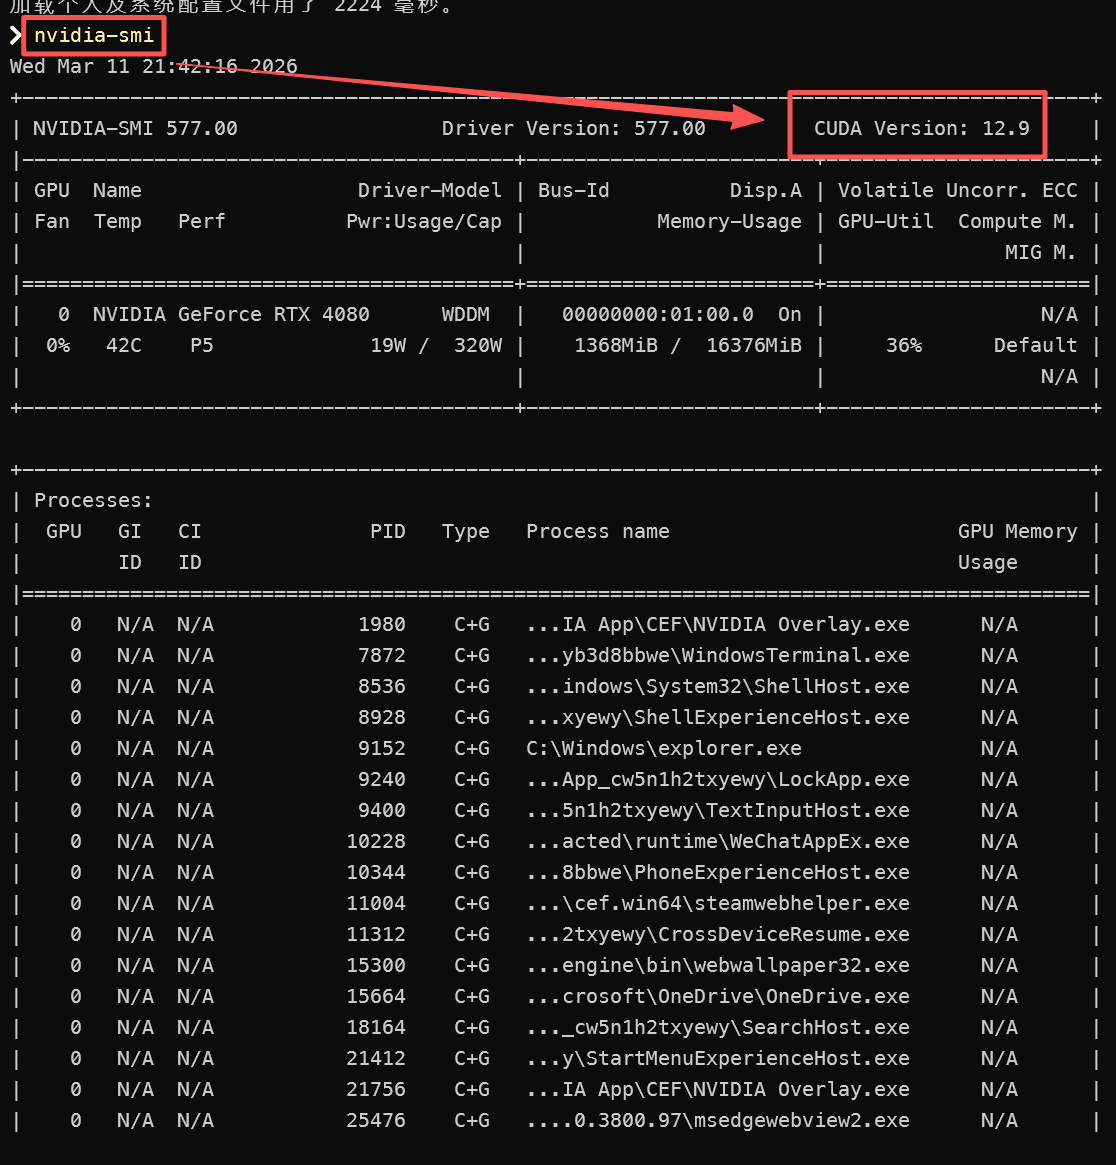
\includegraphics[width=0.7\textwidth]{nvidia-smi.png}
    \end{figure}

\end{frame}

\begin{frame}
    \frametitle{SSH}

    \begin{itemize}
        \item Windows安装：设置，应用，可选功能，添加功能，OpenSSH客户端（你连别人），OpenSSH服务器（别人连你，可以不装）；Mac/Linux自带
        \item \texttt{ssh-keygen}，id25519：椭圆曲线（比RSA：大数分解更好的算法）生成公钥和私钥
        \item 公钥，私钥（这里的钥应当读“月”，只有“钥匙”里读“药”）
        \item \texttt{ssh-copy-id} 复制公钥到服务器（windows没有，必须手动复制，复制到哪一会再说）
        \item \texttt{ssh@hostname} 连接服务器（暂时用不上）
    \end{itemize}
    

\end{frame}

\begin{frame}
    \frametitle{带着玩Linux}

    Clab：\url{clab.pku.edu.cn}

    \begin{itemize}
        \item 登录使用
        \item 创建云主机，playground p2级实例，系统选Ubuntu 24，网络选PKU-new，系统盘30GiB（也就是最小值），其他全都不用管。
        \item \textbf{校园网网络安全性堪忧}，所以不要使用密码，使用密钥。公钥复制进去。\textbf{别复制私钥}。
        \item 等一分钟（云主机创建需要时间）
        \item \texttt{ssh ubuntu@<ip-address>} 连接云主机。你要是开了个大实例，甚至可以用Code连接（略，这个需要在远端安装VS Code Server，慢的一批）。
        \item 问就填yes
    \end{itemize}

\end{frame}

\begin{frame}
    \frametitle{初来乍到}
    \begin{itemize}
        \item 多用户系统，用户之间相互隔离，安全性更好。
        \item 基本思想：一切皆文件 \texttt{cd /dev}
        \item 家目录是\texttt{/home/ubuntu}，或\texttt{\textasciitilde}（一个东西）
        \item 不要把太多东西放在家目录里，\texttt{/tmp}是个好地方，重启就没了。或者你也可以自己搞个文件夹。
        \item \texttt{pwd}，\texttt{ls}（\texttt{exa} 和 \texttt{lsd}），\texttt{whoami}，\texttt{clear}
        \item \texttt{cd}，\texttt{touch}，\texttt{mkdir}，\texttt{rm}，\texttt{cp}，\texttt{mv}，\texttt{echo}
        \item \texttt{cat}（\texttt{bat}），\texttt{grep}
        \item \texttt{scp}，\texttt{rsync}
        \item 新的公钥放在\texttt{.ssh/authorized\_keys}里，一行一个，\texttt{ssh-copy-id}就是帮你搞这个的
    \end{itemize}
\end{frame}

\begin{frame}
    \frametitle{玩}

    \begin{itemize}
        \item \texttt{sl}，\texttt{cmatrix}，\texttt{yes}（\texttt{yes "hello world"}），Ctrl+C
        \item \texttt{fortune | cowsay} （管道，fortune-mod），\texttt{echo "hello" > hello.txt}（重定向）
        \item \texttt{figlet "dabendan"}，\texttt{toilet -f mono12 "dabendan"}
        \item \texttt{fastfetch}, \texttt{neofetch}, \texttt{screenfetch}
        \item \texttt{oneko} \&（\&：后台）；\texttt{bg}，\texttt{fg}，\texttt{jobs}，\texttt{killall oneko}
        \item 设备也是文件，故而可以 \texttt{echo "bendan" > /dev/null} 。null读“闹”就行了
        \item \texttt{/dev}下好玩的东西（不要试图删除或修改它们）：\texttt{null}，\texttt{zero}，\texttt{random}，\texttt{urandom}，\texttt{tty}，\texttt{full}
    \end{itemize}

\end{frame}

\end{document}